\section{Inter Cell Radio Resource Management}
{
	This deals with the problem of \enquote{intercell interference}\cite{Choi2010} and can also be called intercell coordination. This is a growing problem because of greater uses of less powerful cells which cover smaller areas. This allows for the same frequencies to be reused. One of the larger problems in this area is the cell edge performance \enquote{ there is considerable intercell (co-channel) interference from reusing the same frequency channels between neighboring cells. In such interference limited systems, the cell-edge users are more susceptible to this inter-cell interference because, in addition to the high path loss, multiple strong interferences exist from nearby cells.}\cite{InterCellInterferenceCoordination6392819}. The task at hand here is to reduce the interferance for users at the cell edge or in other words optimise network conditions for those users.
	\subsection{OFDMA and SC-FDMA}
	{
		OFDMA is used for the downlink and SC-FDMA for the uplink, both support MIMO antenna systems and using these two technologies allow for bandwidth to be assigned on both a frequency and power. This means that these can be varied to allow users at the cell edge better performance.
	}
	\subsection{Intercell Interference Coordination (ICIC)}
	{
		\Cref{fig:ICICTechniques} shows the three different ways in which performance is improved for users at the cell edge. This involves using the frequency and power features of OFDMA and SC-FDMA to improve conditions and also reducing interference by managing the power and frequency choice for interfering connections.
		\begin{figure}
			\centering
			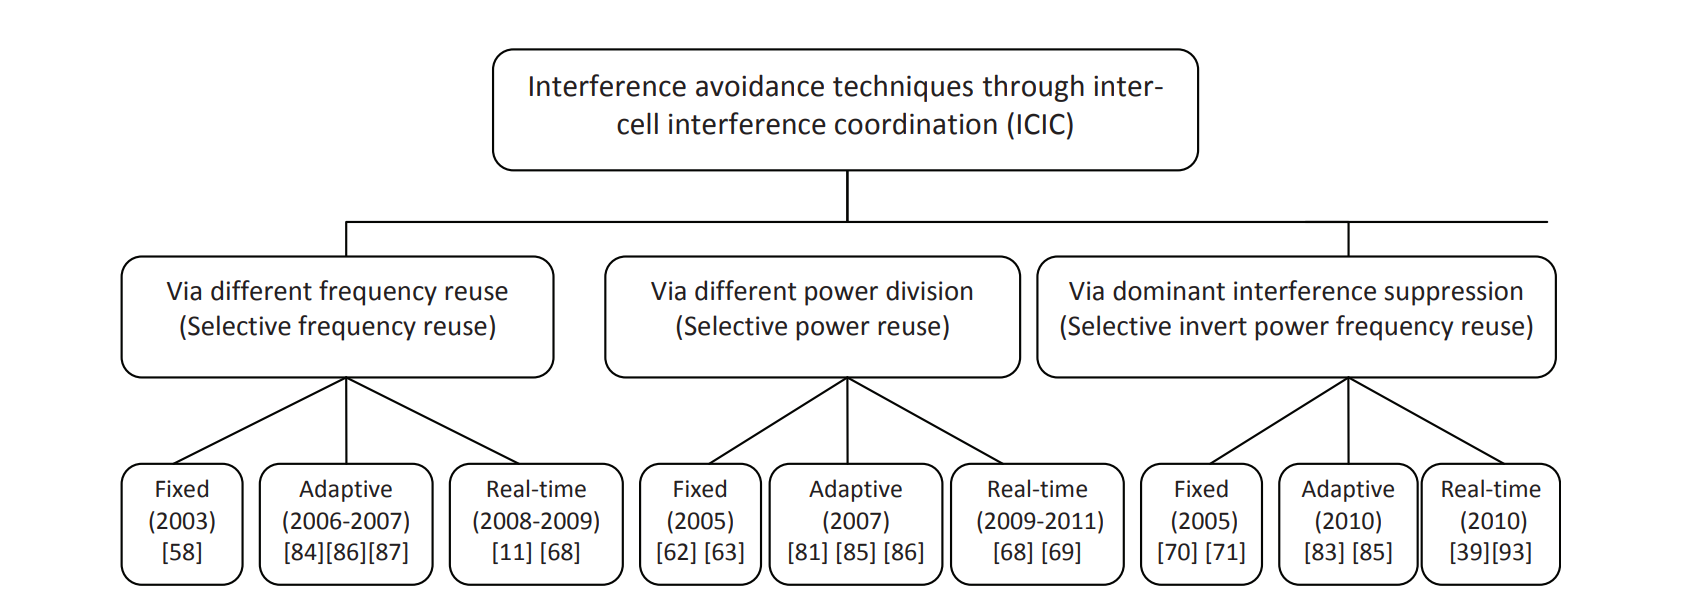
\includegraphics[width=\textwidth]{ICICRRMTechniques}
			\caption{Showing the three ways in which inter-cell interference is managed. \cite{InterCellInterferenceCoordination6392819}}
			\label{fig:ICICTechniques}
		\end{figure}
	}
}